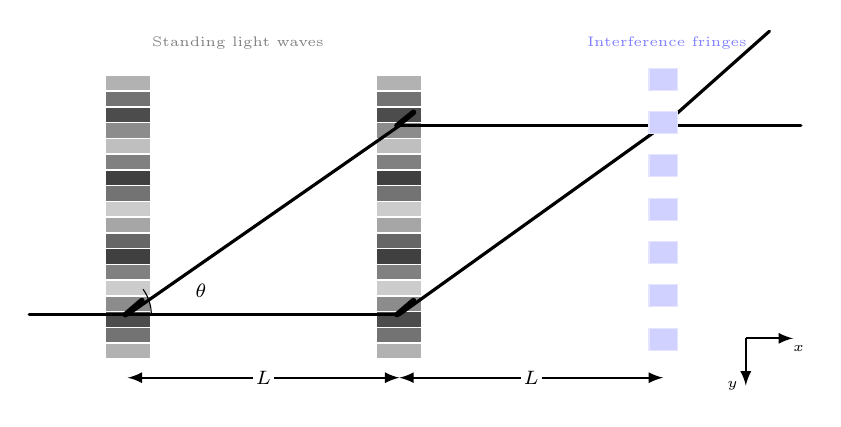
\begin{tikzpicture}[
  x=1cm,y=1cm,
  ray/.style={line width=1.15pt,line cap=round},
  dim/.style={latex-latex,line width=0.8pt},
  label/.style={font=\scriptsize},
  smalllabel/.style={font=\tiny},
  fringe/.style={fill=blue!18,draw=blue!10}
]
  \def\gA{1.30}
  \def\gB{4.75}
  \def\scr{8.10}

  % \node[smalllabel,font=\scriptsize\bfseries] at (4.60,5.85) {Mach--Zehnder interferometer};
  \node[smalllabel,black!50] at (2.70,4.90) {Standing light waves};
  \node[smalllabel,blue!50] at (8.15,4.90) {Interference fringes};

  \foreach \x in {\gA,\gB}{
    \foreach \y/\shade in {0.90/30,1.10/55,1.30/70,1.50/45,1.70/20,1.90/50,2.10/75,2.30/60,2.50/35,2.70/20,2.90/55,3.10/75,3.30/50,3.50/25,3.70/45,3.90/70,4.10/55,4.30/30}{
      \fill[black!\shade] (\x-0.28,\y) rectangle (\x+0.28,\y+0.18);
    }
  }

  \draw[ray] (0.05,1.45) -- (\gA,1.45);
  \draw[ray] (\gA,1.45) -- (\gB,3.85);
  \draw[ray] (\gB,3.85) -- (\scr,3.85);
  \draw[ray] (\gA,1.45) -- (\gB,1.45);
  \draw[ray] (\gB,1.45) -- (\scr,3.85);
  \draw[ray] (\scr,3.85) -- (9.85,3.85);
  \draw[ray] (\scr,3.85) -- (9.45,5.05);

  \draw[ray,line width=2pt] (\gA-0.03,1.45) -- (\gA+0.18,1.63);
  \draw[ray,line width=2pt] (\gB-0.03,1.45) -- (\gB+0.18,1.63);
  \draw[ray,line width=2pt] (\gB-0.03,3.85) -- (\gB+0.18,4.02);

  \draw[thin] (\gA+0.30,1.45) arc[start angle=0,end angle=36,radius=0.55];
  \node[label] at (\gA+0.93,1.76) {$\theta$};

  \foreach \y in {1.00,1.55,2.10,2.65,3.20,3.75,4.30}{
    \path[fringe] (\scr-0.18,\y) rectangle (\scr+0.18,\y+0.28);
  }

  \draw[dim] (\gA,0.65) -- (\gB,0.65);
  \node[label,fill=white,inner sep=1pt] at ({(\gA+\gB)/2},0.65) {$L$};
  \draw[dim] (\gB,0.65) -- (\scr,0.65);
  \node[label,fill=white,inner sep=1pt] at ({(\gB+\scr)/2},0.65) {$L$};

  \draw[-latex,line width=0.8pt] (9.15,1.15) -- (9.75,1.15);
  \draw[-latex,line width=0.8pt] (9.15,1.15) -- (9.15,0.55);
  \node[smalllabel] at (9.82,1.02) {$x$};
  \node[smalllabel] at (8.98,0.55) {$y$};
\end{tikzpicture}